\documentclass[12pt]{article}
\usepackage{geometry}
\usepackage{enumerate}
\usepackage{amsmath}
\usepackage{amssymb}
\usepackage{etoolbox}
\usepackage{graphicx}
\usepackage{framed}
\usepackage{hyperref}

\newcommand{\AND}{\wedge}
\newcommand{\OR}{\vee}
\newcommand{\NOT}{\neg}
\newcommand{\TURN}{\vdash}
\newcommand{\IMPLIES}{\rightarrow}
\newcommand{\IFF}{\leftrightarrow}

\newtheorem{definition}{Definition}
\newcommand{\DoNotShare}{\large \noindent \textbf{Under the Harvey Mudd Honor Code, this document is not to be shared.} \normalsize}
\newcommand{\Problem}[3]{\mbox{} \newline \noindent \textbf{\textbf{Problem #1: #2 [#3 Points] \\ }}}
\newcommand{\WT}[1]{\begin{framed} \noindent \textbf{What's the Rationale?} #1 \end{framed}}

\begin{document}

\begin{center}
	\bf
	CS 81, Logic and Computability  \\
	Problem Set 2:  Natural Deduction for Propositional Logic \\
\end{center}

%\DoNotShare

Problems 1--8 are natural deduction proofs.
In Problems 1--6, you'll use constructive logic.  In Problems 7 and 8, you'll use classical logic which allows the use of RAA (Reductio ad Absurdum), which is also called Proof by Contradiction or Indirect Proof (IP).

Please write your proofs for those problems using the online natural deduction proof checker at \href{http://proofs.openlogicproject.org}{proofs.openlogicproject.org}.  The proof checker will show you that your proof is correct and give you a smiley face.  Take a screenshot of the proof (e.g, using the Grab utility on a Mac or a similar tool) and submit a PDF version of the snapshot with the complete proof and the smiley face that shows that the proof checker verified the correctness of your proof.

Take a few minutes to look at the notation used by the \href{http://proofs.openlogicproject.org}{\texttt{openlogicproject}} online proof checker.  The notation for the ``Rules'' are shown on the right side of the page (you only need the ``Basic Rules'')  and the notation for the operators (and, or, not, implication) are shown on the left side under ``Instructions.''  I suggest that you try to  type in one or two proofs from class in this environment before you start trying your own new proofs.  This environment takes just a bit of practice.  I also strongly encourage you to do these sequent proofs \emph{on paper} before you enter them into the proof checker.  As we saw in class, it's generally helpful to derive these proofs non-linearly, working backwards when necessary to ultimately get to our goal.  It's much easier to do that first on paper and then, afterwards, enter the proof online to be checked.

Here are a few things to keep in mind:
\begin{itemize}
	\item When using AND or OR introduction, you don't specify whether it's left or right introduction.  That makes things a bit easier! 
	\item There are several different choices of symbols that you can use for the logic operators (e.g., and, or, not, implication).
\end{itemize}

\Problem{1}{}{10}

Use natural deduction for \textbf{constructive logic}  in the \href{http://proofs.openlogicproject.org}{\texttt{openlogicproject}} to prove  that:  $A \AND (B \OR C) \TURN (A \AND B) \OR (A \AND C)$.\\

\bf{Answer:} 
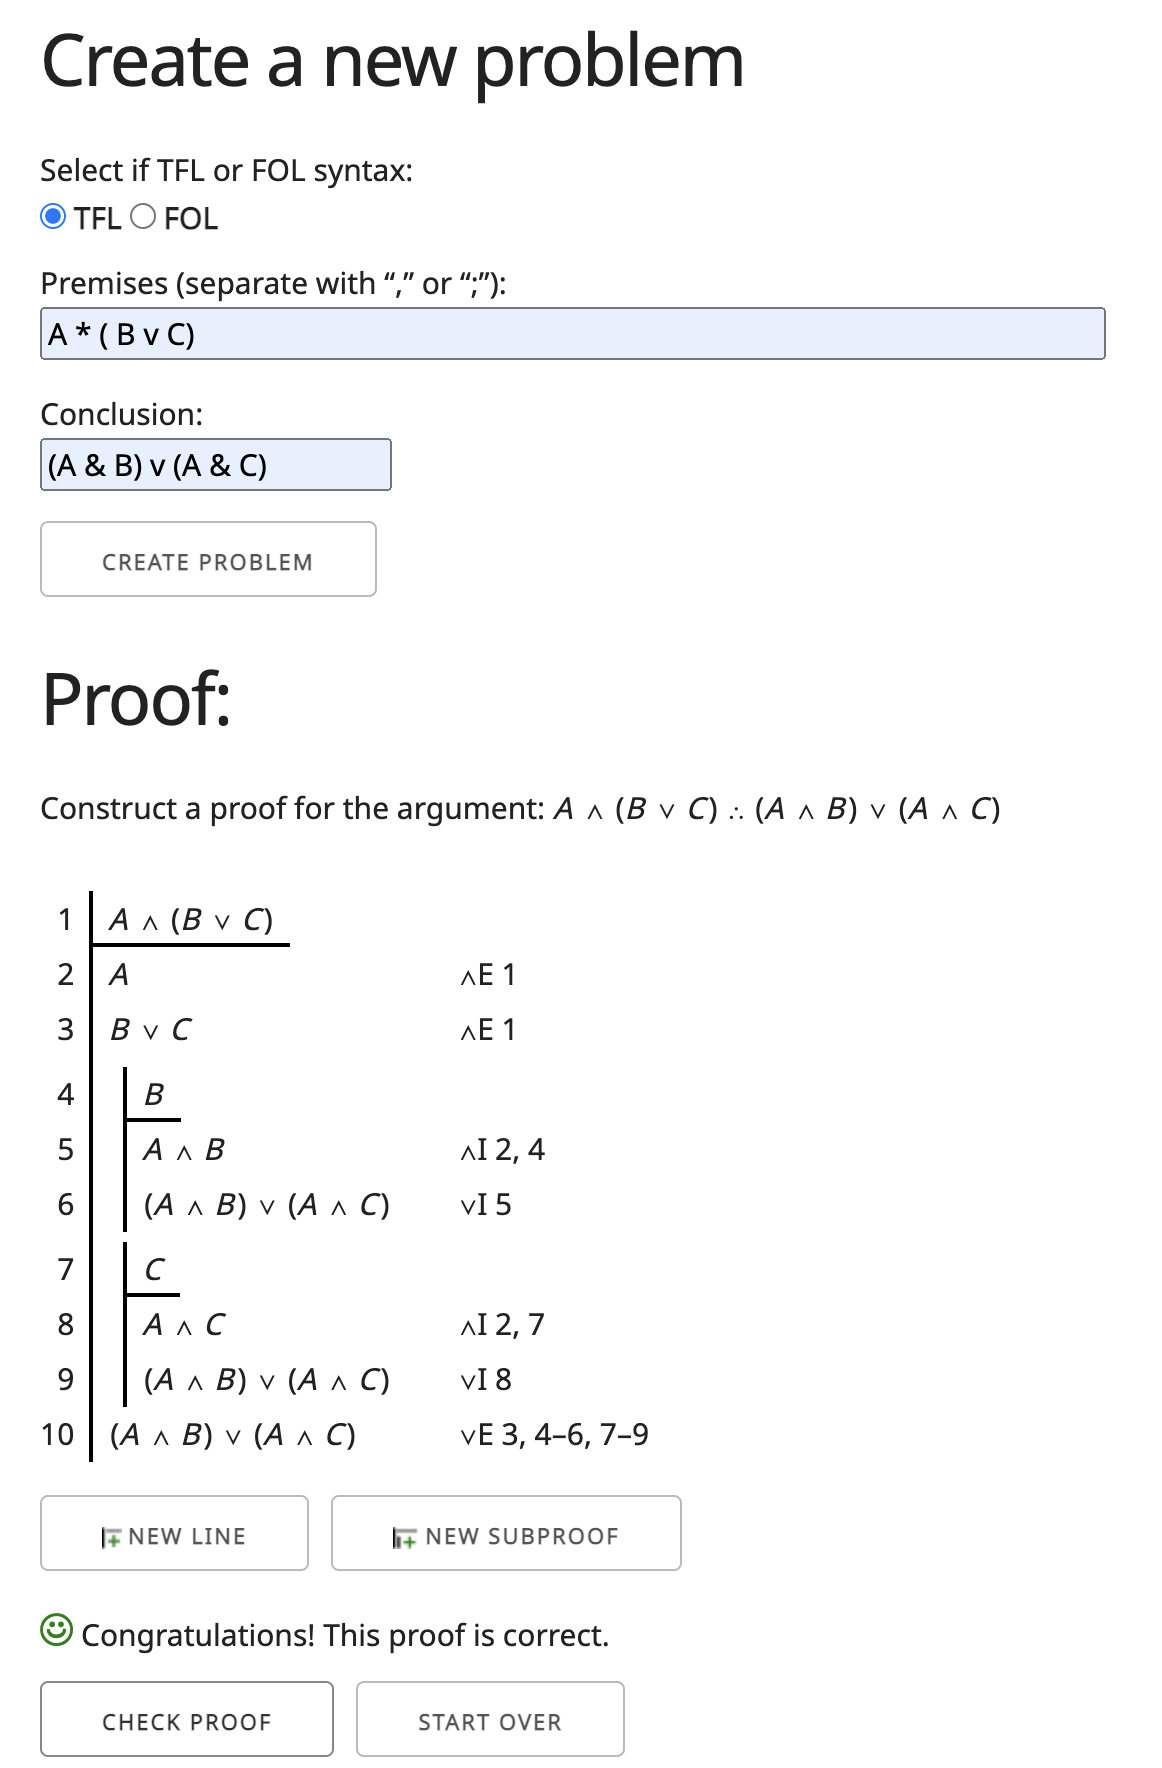
\includegraphics[scale = 0.4]{hw2pr1.png}

\Problem{2}{}{10}

Use natural deduction for \textbf{constructive logic}  in the \href{http://proofs.openlogicproject.org}{\texttt{openlogicproject}} to prove that:  $B \IMPLIES A \TURN (A \IMPLIES C) \IMPLIES (B \IMPLIES C)$.

\bf{Answer:}
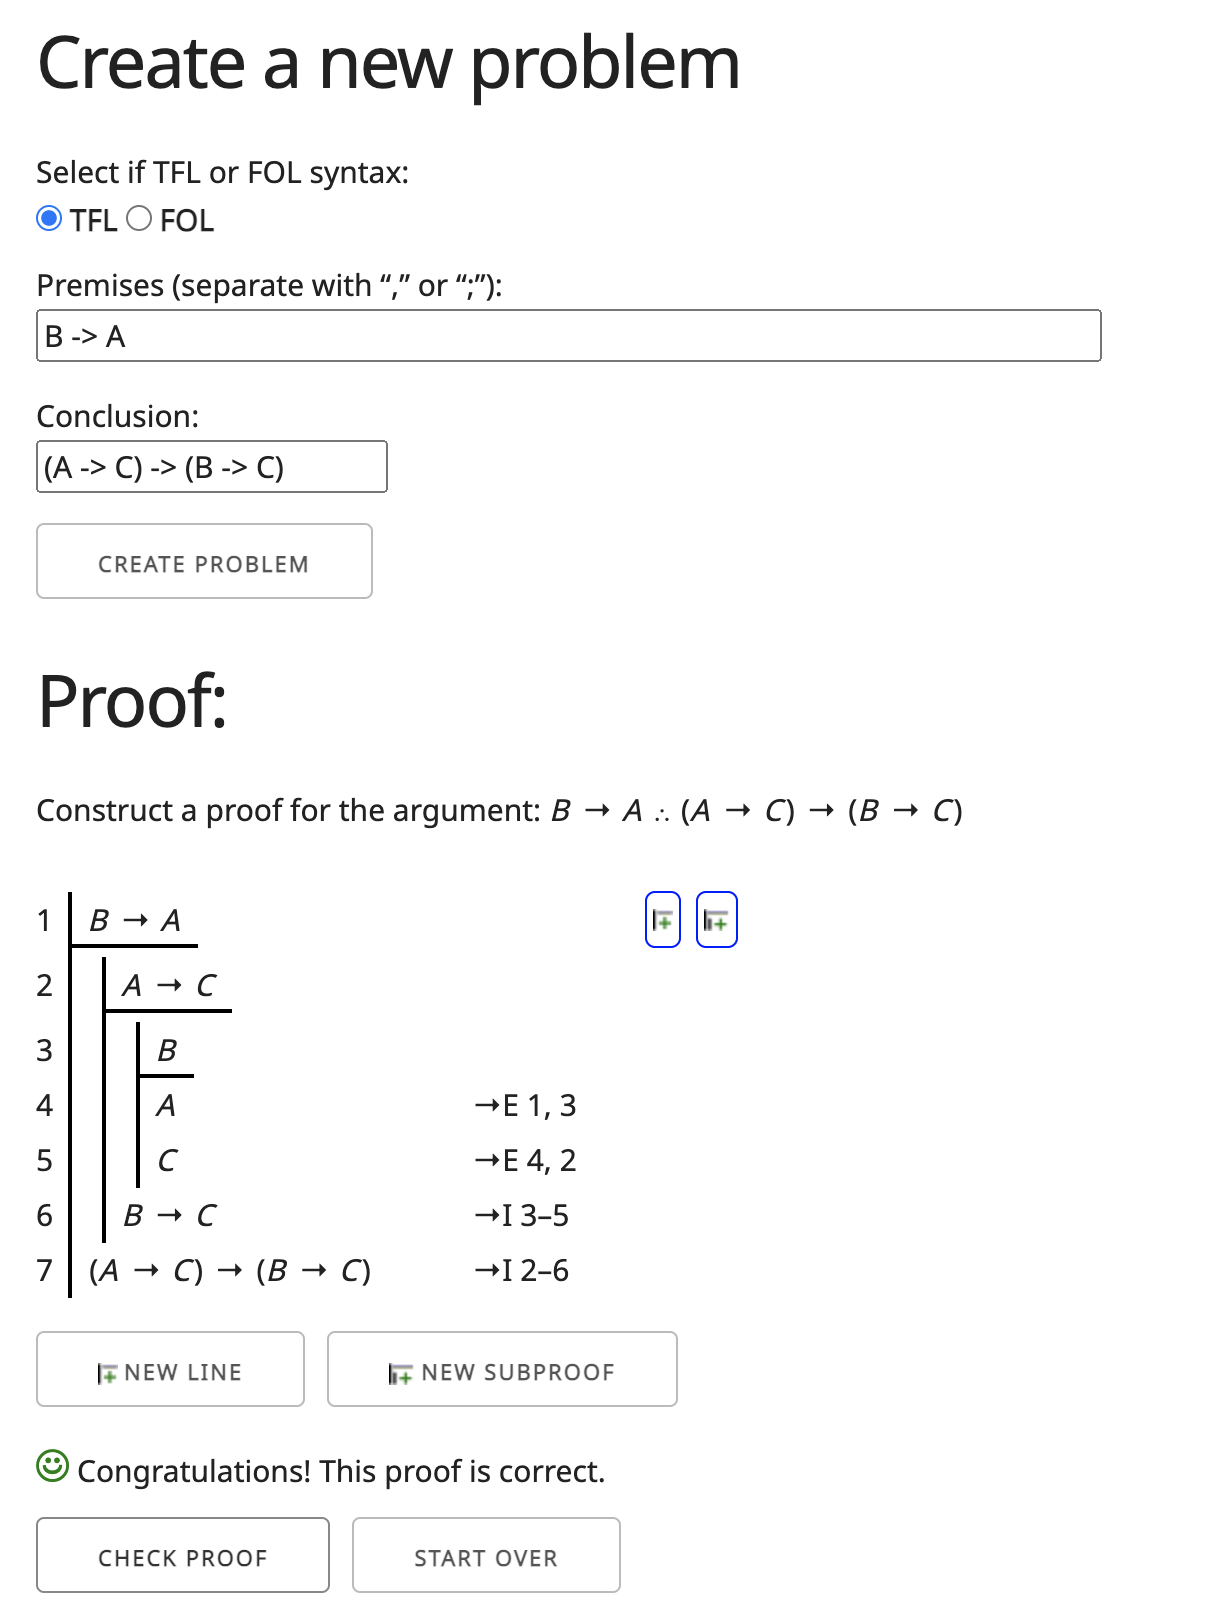
\includegraphics[scale = 0.4]{hw1pr2.png}
\Problem{3}{}{10}

Use natural deduction for \textbf{constructive logic}  in the \href{http://proofs.openlogicproject.org}{\texttt{openlogicproject}} to prove that:  $A \IMPLIES \neg B \TURN B \IMPLIES \neg A$.

\bf{Answer:}
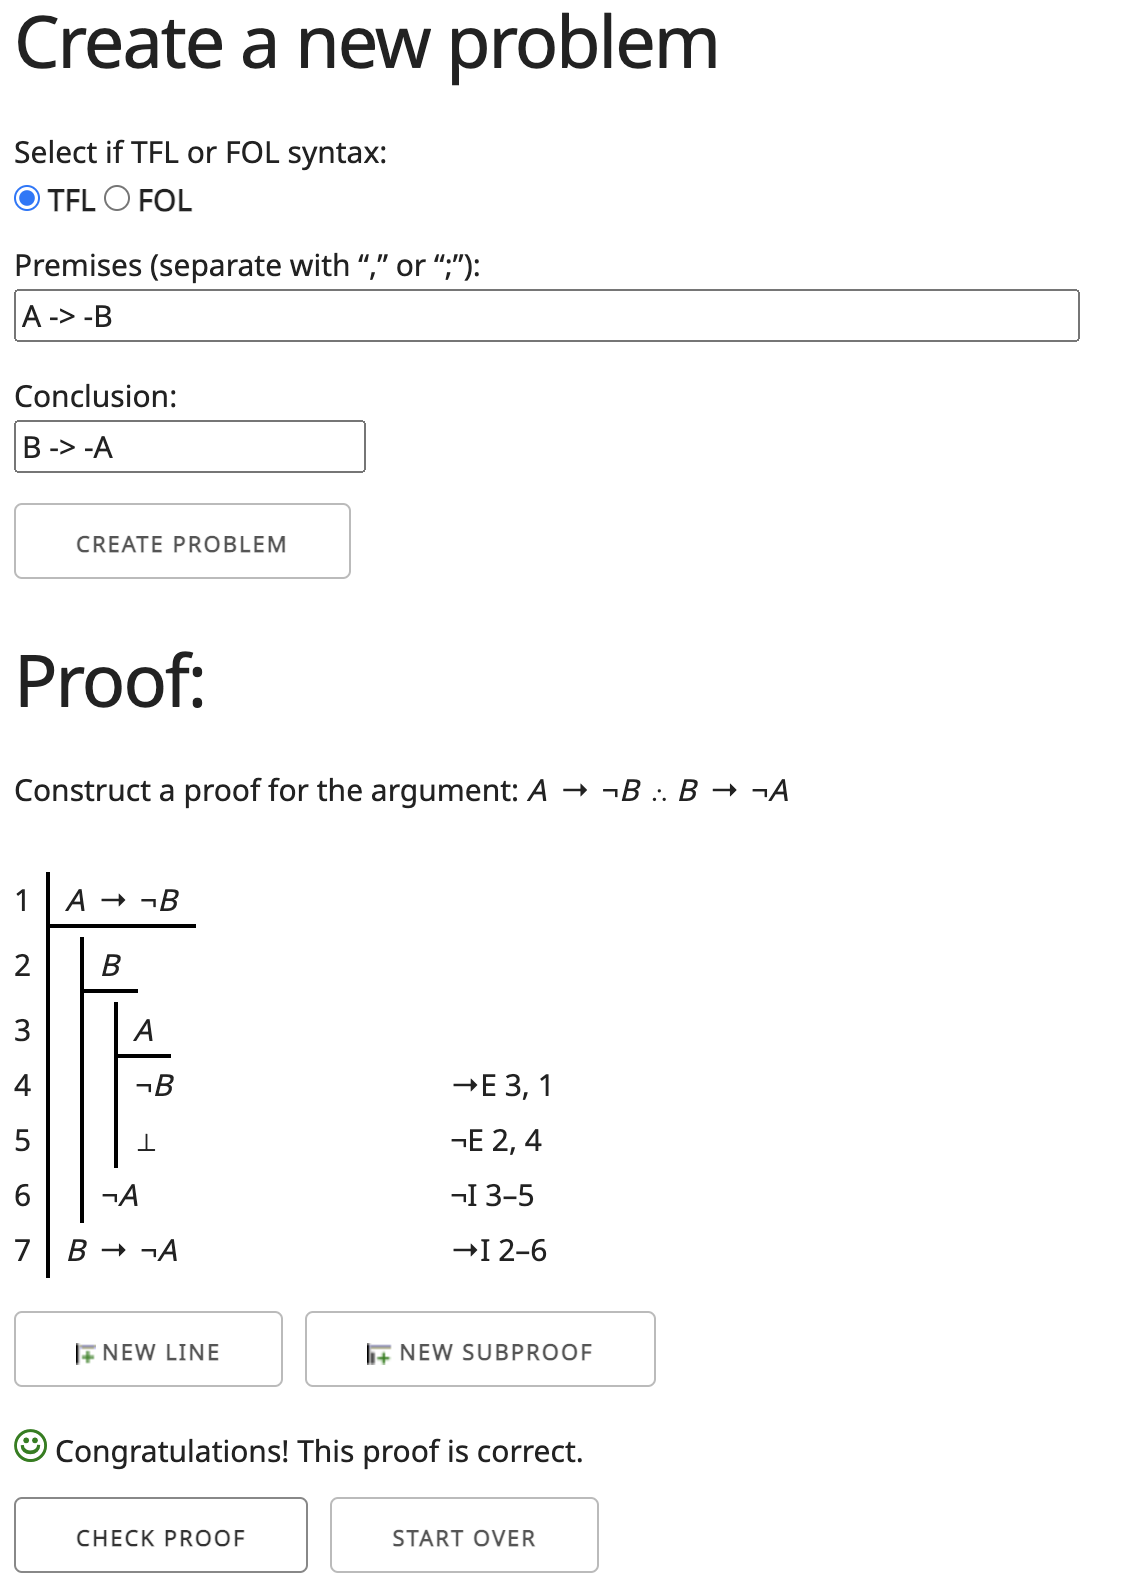
\includegraphics[scale = 0.4]{hw2pr3.png}

\Problem{4}{}{10}

Use natural deduction for \textbf{constructive logic}  in the \href{http://proofs.openlogicproject.org}{\texttt{openlogicproject}} to prove  that:  $\neg \neg \neg A \TURN \neg A$.  (Remember, this is constructive logic.  We have no rule that eliminates a double negative!)

\bf{Answer:}
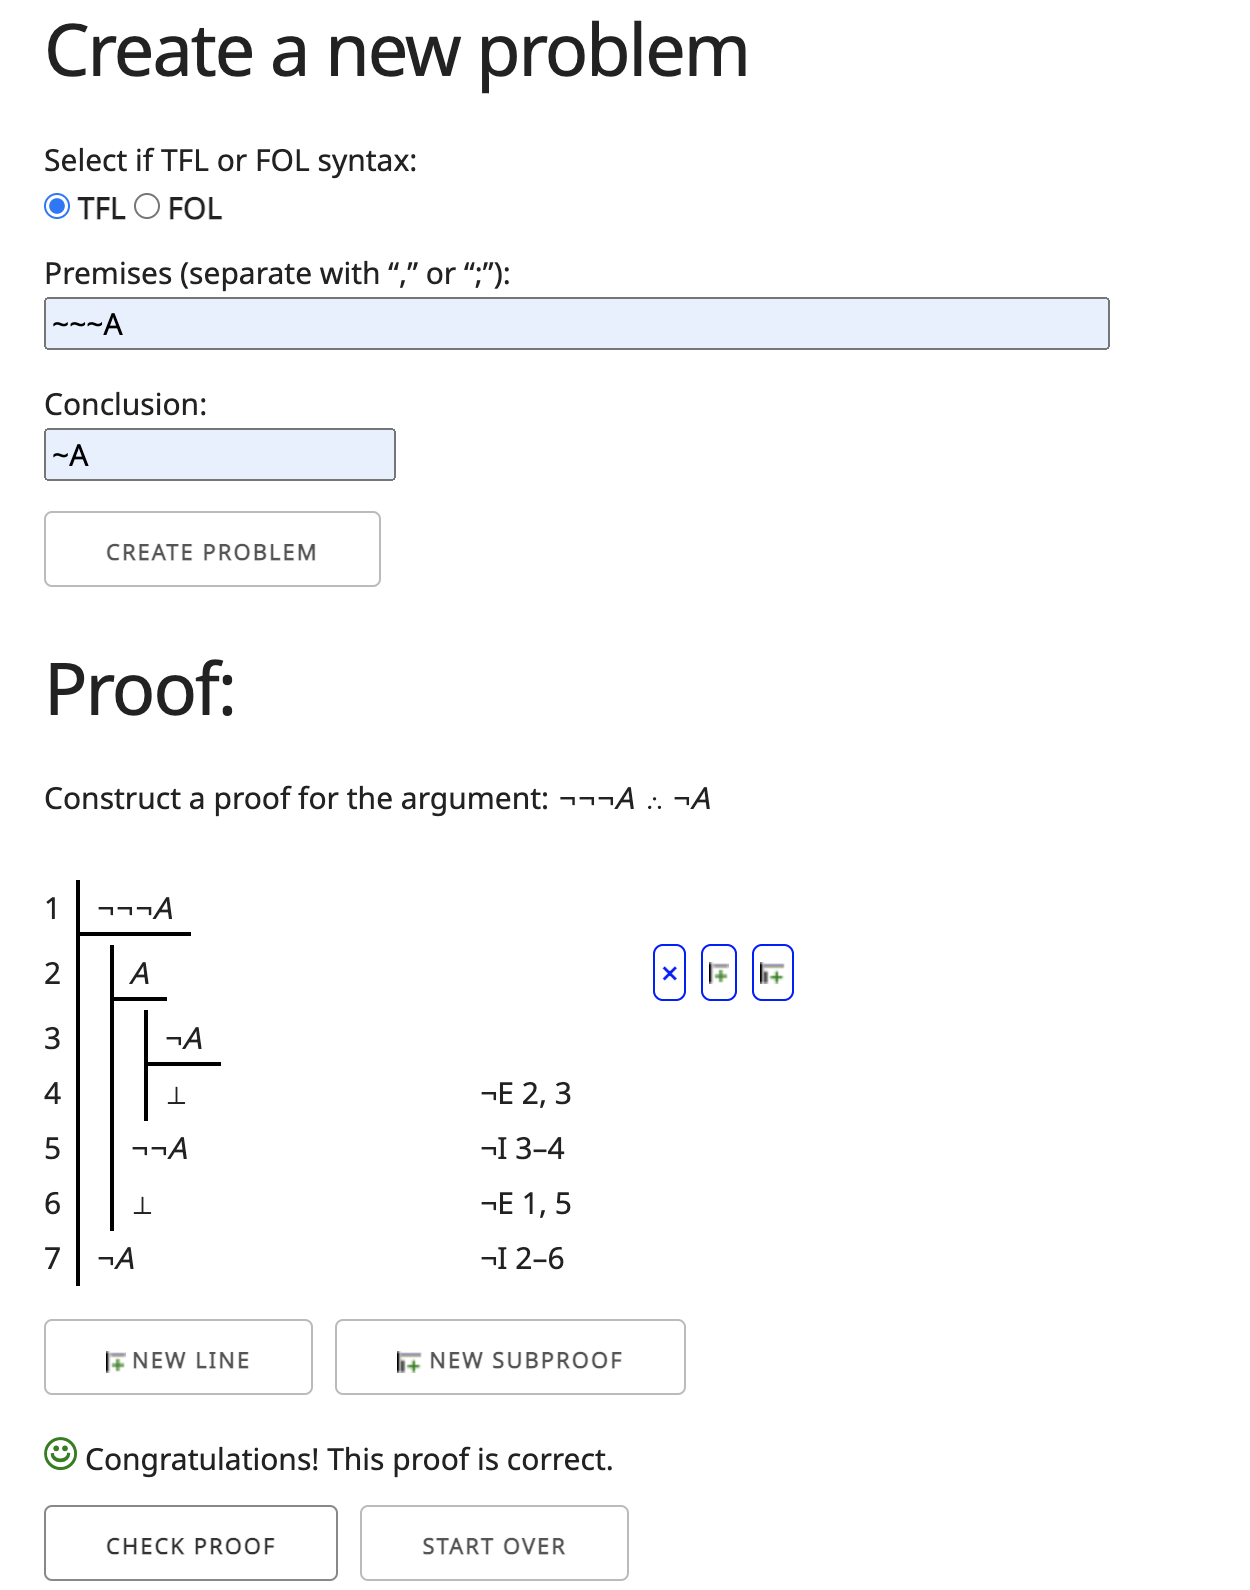
\includegraphics[scale = 0.4]{hw2pr4.png}

\Problem{5}{}{10}

Use natural deduction for \textbf{constructive logic}  in the \href{http://proofs.openlogicproject.org}{\texttt{openlogicproject}} to prove  that:  $A \IMPLIES \neg A \TURN \neg A$.

\bf{Answer:}
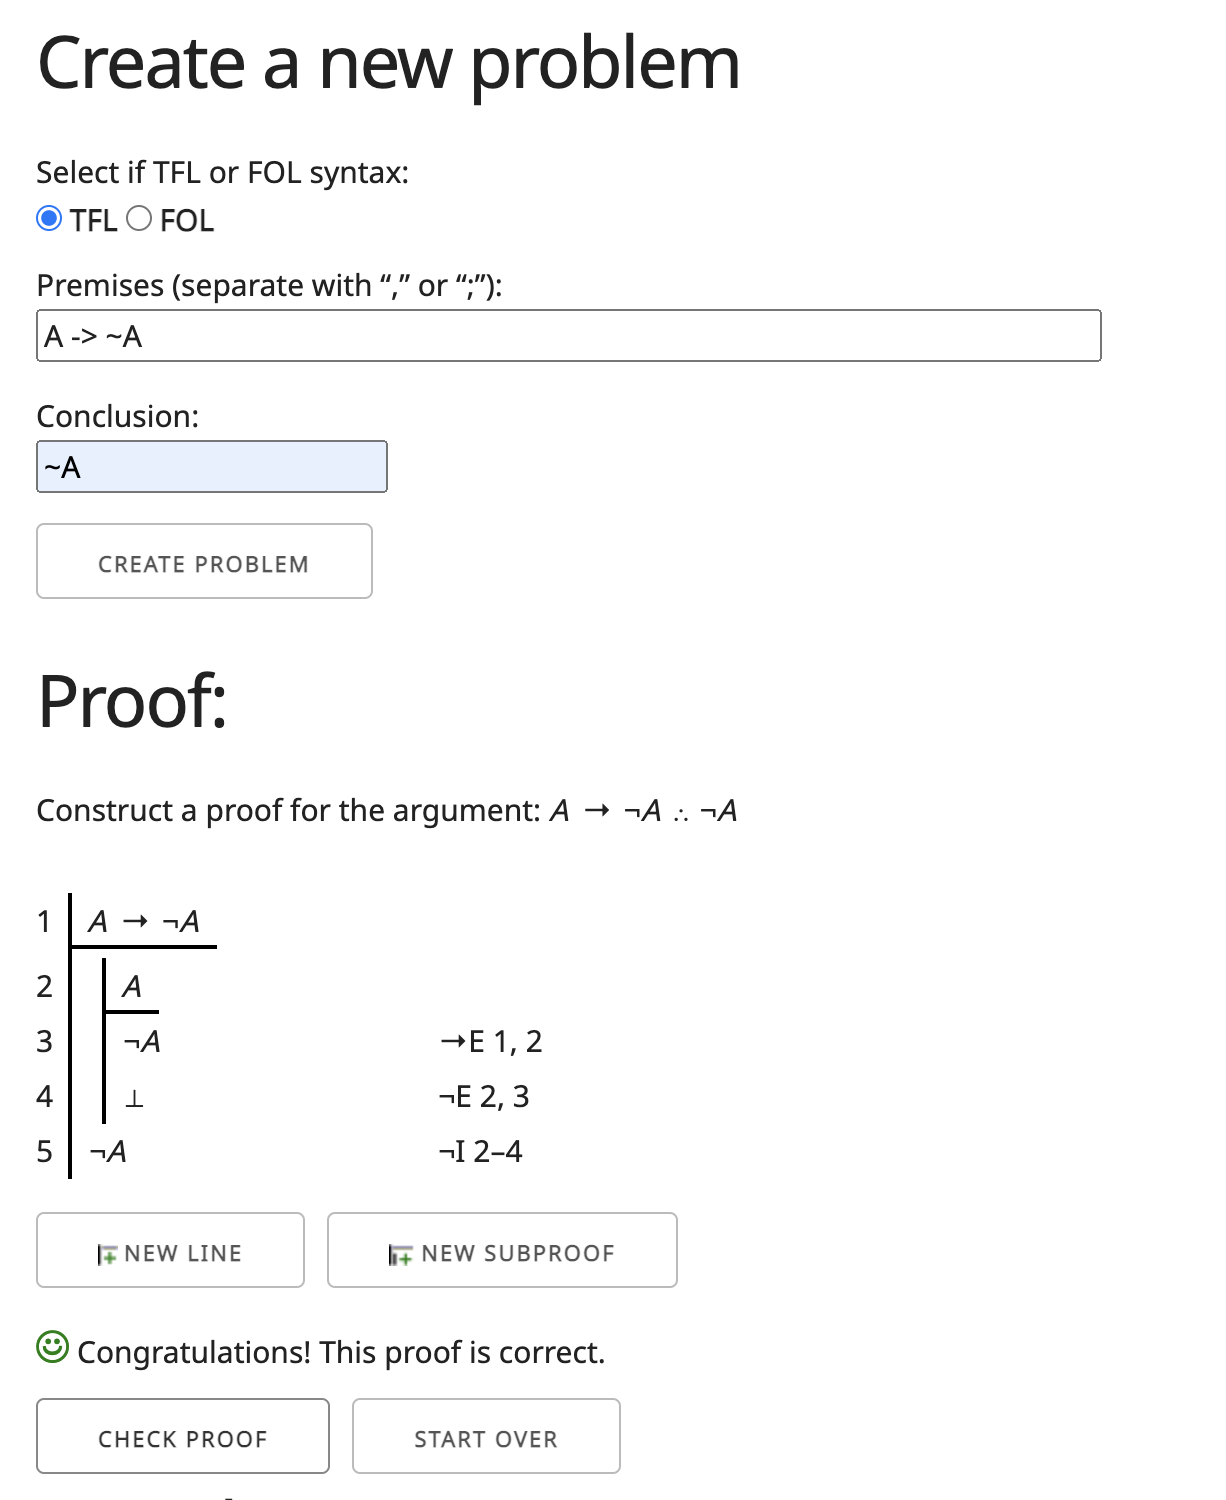
\includegraphics[scale = 0.4]{hw2pr5.png}

\Problem{6}{}{10}

Use natural deduction for \textbf{constructive logic}  in the \href{http://proofs.openlogicproject.org}{\texttt{openlogicproject}} to prove  that:  $A \OR B \TURN \neg( \neg A \AND \neg B)$.

\bf{Answer:}
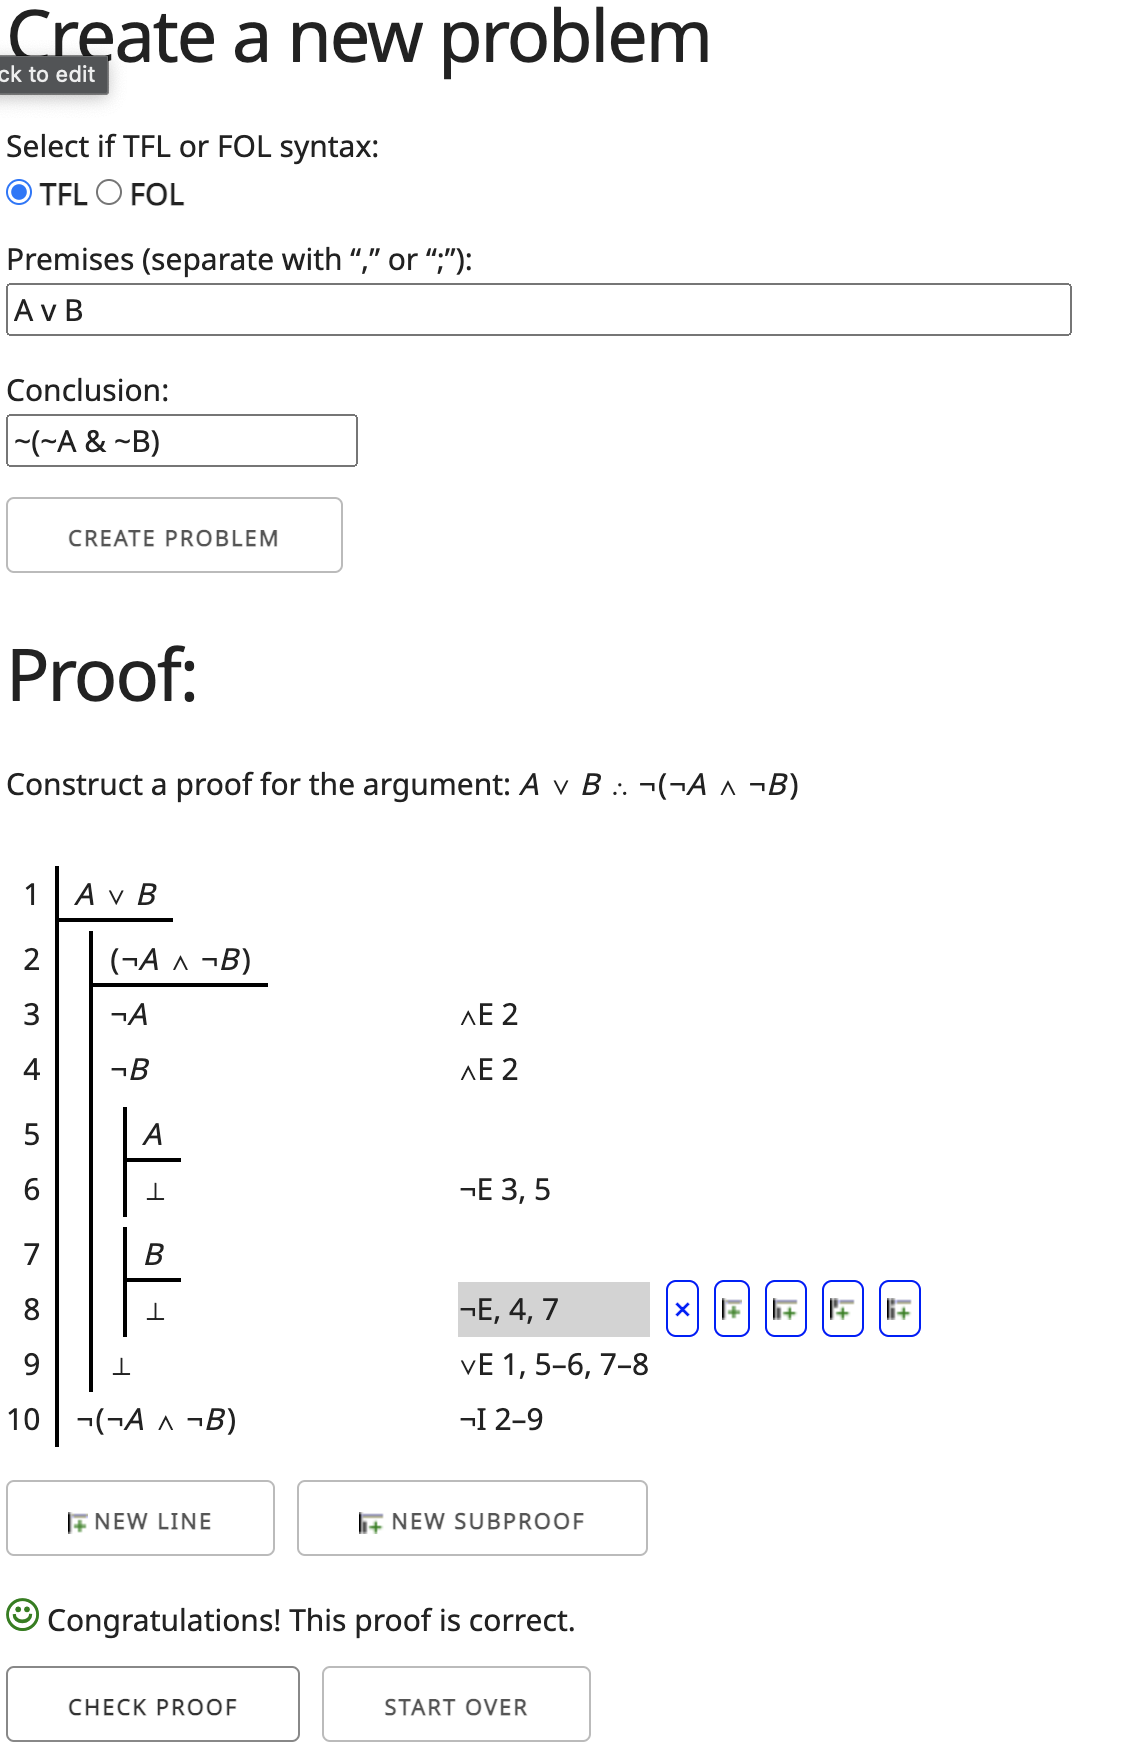
\includegraphics[scale = 0.4]{hw2pr6.png}

\Problem{7}{}{10}

Use natural deduction for \textbf{classical logic} in the \href{http://proofs.openlogicproject.org}{\texttt{openlogicproject}} to prove  that:  $\neg A \IMPLIES A \TURN A$.  (Note:  Since this is in classical logic rather than constructive logic you may use RAA, called IP in \href{http://proofs.openlogicproject.org}{\texttt{openlogicproject}},  in your proof.  In fact, you will need to use IP here.)

\bf{Answer:}
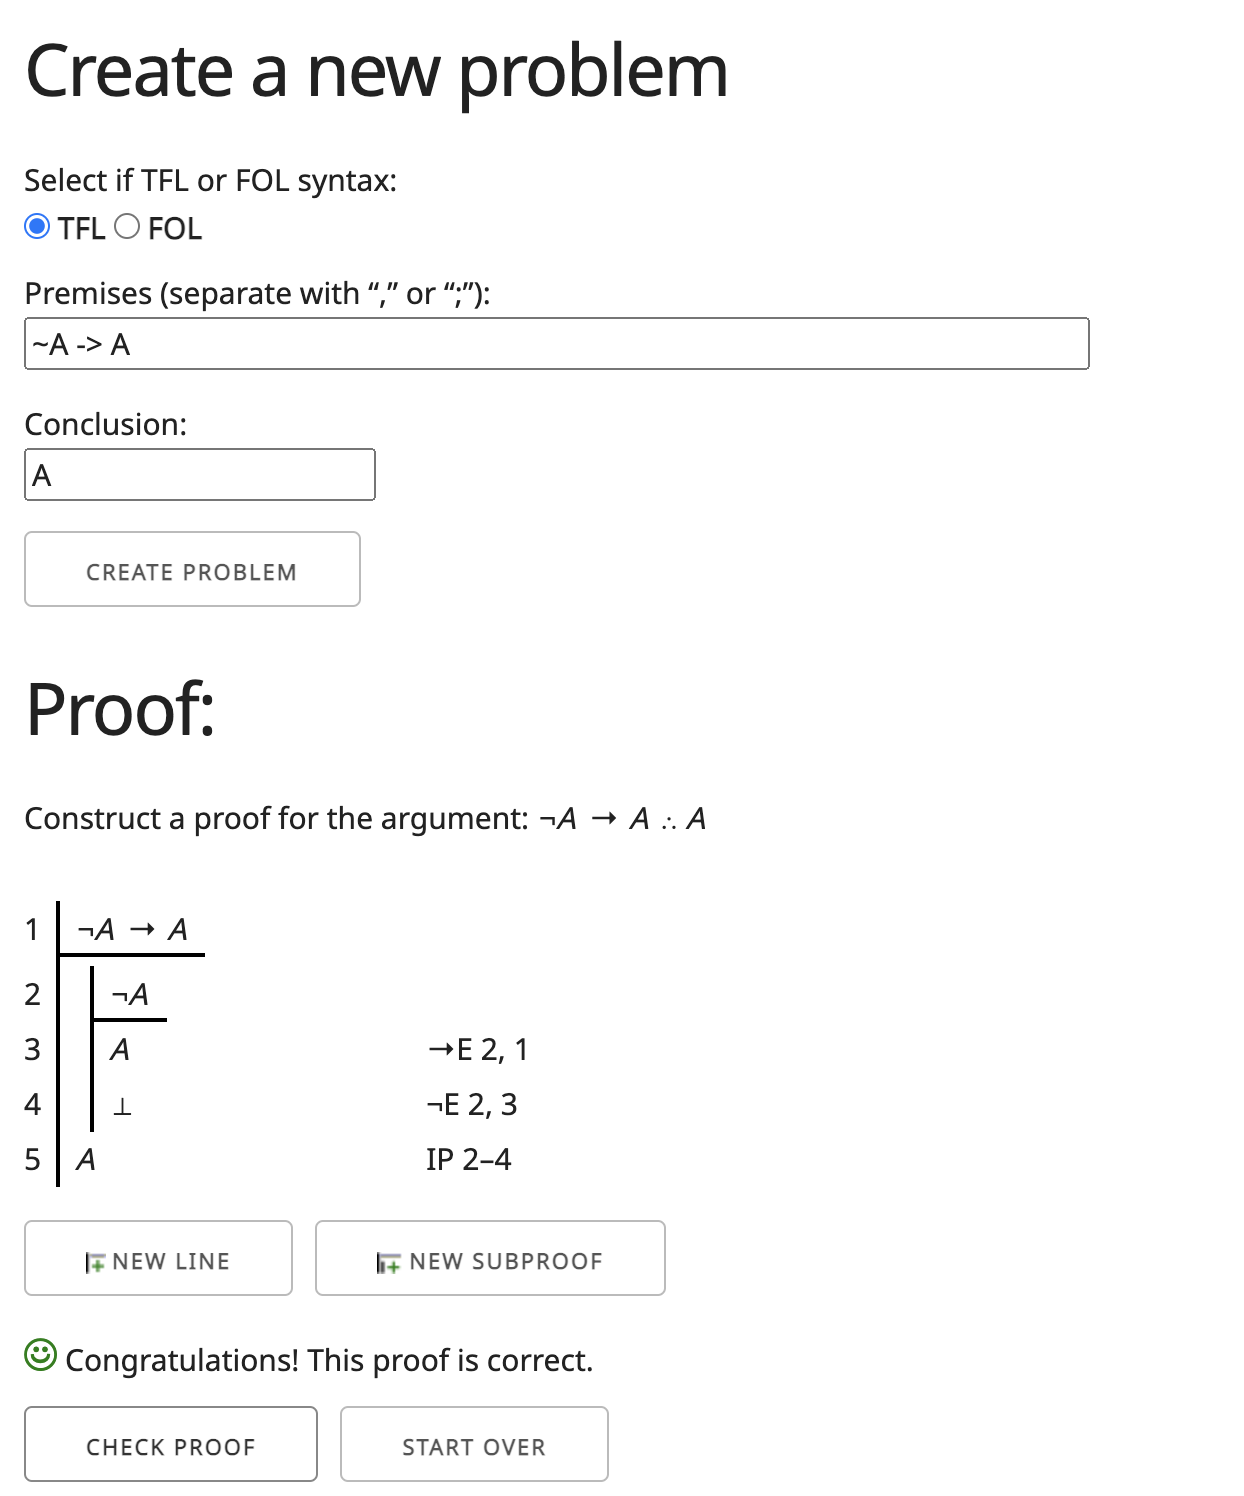
\includegraphics[scale = 0.4]{hw2pr7.png}

\Problem{8}{}{10}

Use natural deduction for \textbf{classical logic} in the \href{http://proofs.openlogicproject.org}{\texttt{openlogicproject}} to prove  that:  $\neg (\neg A \AND \neg B) \TURN A \OR B$.    (Note:  Since this is in classical logic rather than constructive logic you may use RAA, called IP in \href{http://proofs.openlogicproject.org}{\texttt{openlogicproject}}, in your proof.  In fact, you will need to use IP here.)

\bf{Answer:}
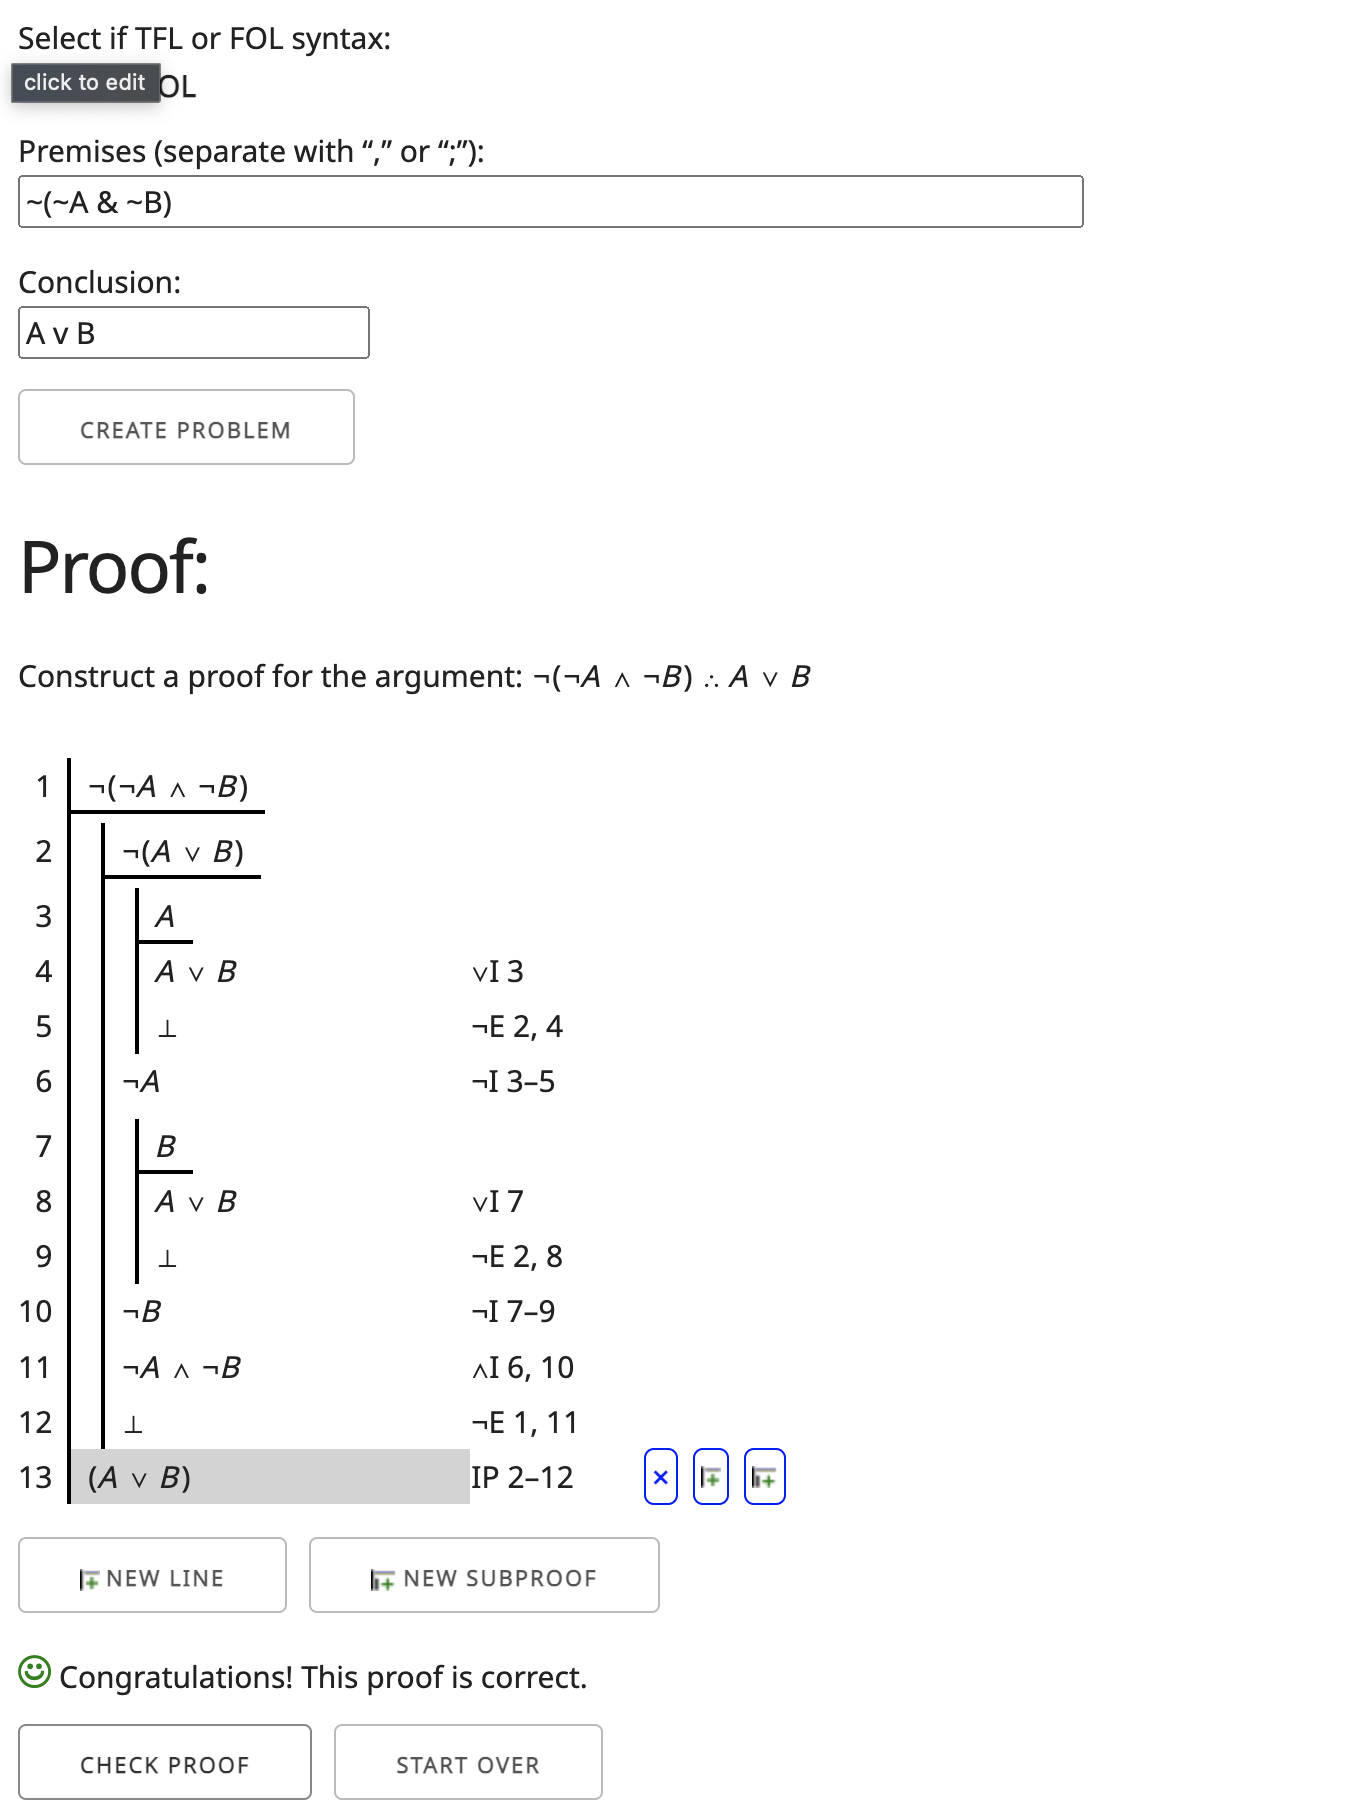
\includegraphics[scale = 0.4]{hw2pr8.png}

\Problem{9}{Knights, Knaves, Gold!}{10}

You are on an island inhabited by knights and knaves. 
You may interact with the inhabitants of this island by only asking questions that can be answered with ``yes'' (true) or ``no'' (false).
Knights always tell the truth and knaves always lie.  

You arrive on the island believing that there may be gold to be found there.  Almost immediately, you encounter an inhabitant.
Your goal is to ask that inhabitant only one question and the answer to that question should tell you whether or not there is gold on the island.

	\begin{enumerate}
		\item What question should you ask?  More precisely, what statement would you present to the inhabitant such that their answer would reveal whether or not there is gold.   For example, if you wanted to ask the question ``Are you a knave and there is no gold on this island?''~you would turn this into a statement ``You are a knave and there is not gold on the island.''
		\item Express your statement in propositional logic by defining a variable for each proposition in your statement and using those variables and logical connectives ($\AND$, $\OR$, $\NOT$, $\IMPLIES$, $\IFF$) to express your statement.   For example, if $p$ = ``you are a knave'' and $q$  = ``there is gold on the island'' then the statement  ``you are a knave and it is not the case that there is gold on the island'' would be written as $p \wedge \NOT q$.
        \item Use a truth table to prove that your question allows you to determine whether or not there is gold on the island. \textbf{Tip:} You can add a column to your truth table showing the inhabitant's response, and use that to show how the responses of the inhabitant allow you to determine precisely whether or not there is gold on the island. In other words, there is the \textit{actual} truth value of your proposed logical statement, determined fully by the settings of the propositional variables, and then there is the response of the inhabitant, which might be different from the actual truth value of your logical statement, depending on whether they are a knight or a knave. You would then show that this response column allows you to determine with full accuracy whether there is gold on the island, no matter if the respondent is a knight or a knave. Also note that a knave does not negate propositions within your logical statement individually, but only negates the entire logical statement in the final step, as a whole. 
	\end{enumerate}

	{\bfseries Answer}\\
	\begin{enumerate}
		\item The statement that one should use would be "there is gold if an only if you are a knight".
		\item Let $p$ be the statement "there is gold" and let $q$ be the statement "you are a knight", we can see then that we can express the statement as $p \IFF q$.
		\item We can construct the following truth table. It is important to note that that when $q=0$, the statement that we are actually evaluating is $\not (p \IFF q)$ since we know that when $q = 0$, we have a knave and that knaves negate the entire statement. Therefore, keeping this is mind, we can construct the following table.
		\begin{center}
			\begin{tabular}{||c c c c||} 
			 \hline
			 $p$ & $q$ & $p \IFF q$ & $\NOT \;(p \IFF q)$ \\ [0.5ex] 
			 \hline\hline
			 0 & 0 & 1 & 0 \\ 
			 \hline
			 1 & 0 & 0 & 1 \\
			 \hline
			 0 & 1 & 0 & 1 \\
			 \hline
			 1 & 1 & 1 & 0 \\
			 \hline
			\end{tabular}
			\end{center}
			We can see that considering our situation, the reality of our situation is reflected in our first two rows adjoined with the second two rows of our table, which we can see gives us truth values of 1 only when there is gold on the island.
	\end{enumerate}
	

\Problem{10}{Monks, Proofs, Transcendence!}{10}

A group of monks live in a monastery. They have taken a vow of silence, and cannot communicate with each other in any way. Each morning, the monks silently enter a large prayer chamber, where they all sit silently facing each other to pray, then return to their own rooms at night. They are expected to pray every day, but if they ever become aware that they have achieved transcendence, they will pack up their belongings in the night and leave the monastery. When a monk achieves transcendence, a luminous mark appears on their forehead. There are no mirrors in the monastery, so each monk cannot see their own forehead, though they do see the foreheads of all of the other monks when they are all in the prayer chamber together. One night (and on that night only!), which we'll call ``night 0'', while all the monks are in their own rooms, a booming voice rings out: ``At least one of you has achieved transcendence!''  The next day is denoted ``day 1.''  You should assume that the monks are good at logic and will leave at the earliest time that it is possible for them to determine that they have transcended (and, of course, that a non-transcendent monk will not leave).

\begin{enumerate}
	\item State a claim about what day the transcendent monks will leave if there are exactly $n$ transcendent monks.
	\item Prove your claim by induction. 
\end{enumerate}

\bf{Answer:}
\begin{enumerate}
	\item All the transcendent monks would leave on day $n$ if there are exactly $n$ transcendent monks.
	\item Consider the following proof of the claim by induction. \\\\
	Let us first consider the base case of where $n = 1$. We can see trivially that after night 0, the voice booms out and claims that at least one monk has achieved transcendence. However, as there is only one monk, it must follow that said monk is the one who has achieved transcendence, and thus, they leave on day 1. Thus, we have established our base case. \\\\
	Now, let us assume that our inductive hypothesis holds for $n$ monks. We will now prove that the statement holds for $n + 1$ monks. Consider that if we have $n+1$ monks, we can consider that for days 1-n, each monk has insufficient information as to the number of monks who have achieved transcendence. That is, each sees $n$ monks who have the marking for transcendence.
	Using our inductive case, we can see that for $n$ monks, it takes $n$ days for the monks to leave, but now, on the ${n+1}^{th}$ date, each monk realizes that none of the $n$ other monks have left, which indicates that they also see $n$ monks with said marking.
	As a result, each monk realizes that they are indeed also marked and subsequently leave the monastery. Thus, our inductive hypothesis holds for $n+1$ monks as desired.\\\\
	Therefore, as our inductive proof holds for our base case and our inductive step, it follows that our proof holds for all $n$ as desired.
	
\end{enumerate}
\end{document}
